Author: Lester Hedges Email:~~ lester.hedges@bristol.ac.uk

\hypertarget{nodes-interoperable-workflow-components}{%
\section{\texorpdfstring{Nodes: \emph{Interoperable workflow
components}}{Nodes: Interoperable workflow components}}\label{nodes-interoperable-workflow-components}}

The companion notebook for this section can be found
\href{https://github.com/michellab/BioSimSpaceTutorials/blob/4844562e7d2cd0b269cead56562ec16a3dfaef7c/01_introduction/04_writing_nodes.ipynb}{here}

So far we have been working with BioSimSpace in a rather ad hoc fashion.
While this intereactive exploration is a great way of learning and
prototyping ideas, it is not a good way of producing a reproducible and
interoperable script that can be shared with others. For example, we
created processes that used specific packages such as AMBER and GROMACS.
If a user didn't have these available on their system, then the script
simply wouldn't work. We also used hard-coded paths to input files. This
means the user would have to edit the paths each time they ran the
script with different input, which would quickly become tedious.

In order to solve this problem, a core concept of BioSimSpace is the
interoperable workflow component, or \emph{node}. These are robust and
portable Python scripts that typically do a small, well-defined piece of
work. All inputs and outputs from the node are validated and the node is
written in a such a way that it is \emph{independent} of the underlying
software packages, i.e.~the same script can work with a range of
different packages. In addition, nodes are aware of the environment in
which they are run, so can be used interactively, from the command-line,
or within a workflow engine.

While it is possible to write a node directly as a Python script, we
suggest that the best way of writing one is inside of a
\href{http://jupyter.org}{Jupyter} notebook. As you've already seen, the
interactive notebook environment provides a fantastic way of prototyping
and documenting your node and will allow a user to interact with it
directly on a remote cloud server, such as
\href{https://notebook.biosimspace.org}{notebook.biosimspace.org}. The
notebook can provide a complete record of your work, inlcuding
documentation, visualisation, and graphs. When you are happy with the
node, you can download it as a regular Python script (by clicking on
\texttt{File/Download\ As/Python} in JupyterHub or
\texttt{File/Export\ Notebook\ As/Export\ Notebook\ to\ Executable\ Script}
in JupyterLab) and run it directly from the command-line on your
workstation, laptop, or on a high-performance computing cluster. Any
interactive BioSimSpace elements, such as molecular visualisations, will
simply be ignored when run this way.

\hypertarget{an-example-minimisation}{%
\subsection{An example: Minimisation}\label{an-example-minimisation}}

In the rest of the notebook you'll learn how to use BioSimSpace to write
a robust and interoperable workflow node to perform energy minimisation
on a molecular system.

As always, we'll first need to import BioSimSpace:

\begin{Shaded}
\begin{Highlighting}[]
\ImportTok{import}\NormalTok{ BioSimSpace }\ImportTok{as}\NormalTok{ BSS}
\end{Highlighting}
\end{Shaded}

We begin by creating a \texttt{Node} object. This is the core of our
molecular workflow component. It defines what it does, what input is
needed, and the output that is produced.

\begin{Shaded}
\begin{Highlighting}[]
\NormalTok{node }\OperatorTok{=}\NormalTok{ BSS.Gateway.Node(}\StringTok{"A node to perform energy minimisation and save the minimised molecular configuration to file."}\NormalTok{)}
\end{Highlighting}
\end{Shaded}

We'll now set the author and license of the node. When nodes are run the
the authorship can be queried so that people can get credit for their
work. Eventually, BioSimSpace nodes also will also contain built in
tracking information to determine how many times they are run.

\begin{Shaded}
\begin{Highlighting}[]
\NormalTok{node.addAuthor(name}\OperatorTok{=}\StringTok{"Lester Hedges"}\NormalTok{, email}\OperatorTok{=}\StringTok{"lester.hedges@bristol.ac.uk"}\NormalTok{, affiliation}\OperatorTok{=}\StringTok{"University of Bristol"}\NormalTok{)}
\NormalTok{node.setLicense(}\StringTok{"GPLv3"}\NormalTok{)}
\end{Highlighting}
\end{Shaded}

Nodes require inputs. To specify inputs we use the \texttt{BSS.Gateway}
package, which is used as a bridge between BioSimSpace and the outside
world. This will allow us to document the inputs, define their type, and
specify any constraints on their allowed values. Here we will need a set
of files that define the molecular system, and an integer that indicates
the number of minimisation steps to perform.

\begin{Shaded}
\begin{Highlighting}[]
\NormalTok{node.addInput(}\StringTok{"files"}\NormalTok{, BSS.Gateway.FileSet(}
    \BuiltInTok{help}\OperatorTok{=}\StringTok{"A set of molecular input files."}\NormalTok{)}
\NormalTok{)}

\NormalTok{node.addInput(}\StringTok{"steps"}\NormalTok{, BSS.Gateway.Integer(}
    \BuiltInTok{help}\OperatorTok{=}\StringTok{"The number of minimisation steps."}\NormalTok{,}
\NormalTok{    minimum}\OperatorTok{=}\DecValTok{0}\NormalTok{,}
\NormalTok{    maximum}\OperatorTok{=}\DecValTok{1000000}\NormalTok{,}
\NormalTok{    default}\OperatorTok{=}\DecValTok{10000}\NormalTok{)}
\NormalTok{)}

\NormalTok{node.addInput(}\StringTok{"engine"}\NormalTok{, BSS.Gateway.String(}
    \BuiltInTok{help}\OperatorTok{=}\StringTok{"The molecular dynamics engine"}\NormalTok{,}
\NormalTok{    allowed}\OperatorTok{=}\NormalTok{BSS.MD.engines(),}
\NormalTok{    default}\OperatorTok{=}\StringTok{"auto"}\NormalTok{)}
\NormalTok{)}
\end{Highlighting}
\end{Shaded}

Note that the input requirements \texttt{steps} and \texttt{engine} have
default values, so are optional.

We now need to define the output of the node. In this case we will
return a set of files representing the minimised molecular system.

\begin{Shaded}
\begin{Highlighting}[]
\NormalTok{node.addOutput(}\StringTok{"minimised"}\NormalTok{, BSS.Gateway.FileSet(}\BuiltInTok{help}\OperatorTok{=}\StringTok{"The minimised molecular system."}\NormalTok{))}
\end{Highlighting}
\end{Shaded}

When working interactively within a Jupyter notebook we need a way to
allow users to set the input requirements. The
\texttt{node.showControls} method will display a graphical user
interface (GUI), from which inputs can be set. All of the elements for
this GUI are automatically generated by the \texttt{addInput} and
\texttt{addOutput} functions above. As you'll see in the next section,
if we were to run the same node from the command-line, we would instead
get an automatically generated
\href{https://docs.python.org/3/library/argparse.html}{argparse} parser.

Note that the GUI requires active user input. All input requirements
that don't have a default value \emph{must} be set before the node can
proceed. If you try to query the node for one of the user values then an
error will be raised. For bounded integer inputs you can use a slider to
set the value, or type in the input box and press enter.

When working interactively you will typically be running on a remote
server where you won't have access to the local filesystem. In this case
you'll need to upload files for any of the \texttt{File} or
\texttt{FileSet} input requirements. The GUI below will provide buttons
that allow you to browse your own filesystem and select files. Since
Jupyter has a limit of 5MB for file transfers, we provide support for
compressed formats, such as \texttt{.zip} or \texttt{.tar.gz}. (A single
archive can contain a set of files, allowing you to set a single value
for a \texttt{FileSet} requirement.) We've provided some example input
files that can be used in the training notebooks, which are available to
download from the links below. These can then be re-uploaded using the
GUI.

AMBER:
\href{https://raw.githubusercontent.com/michellab/BioSimSpace/devel/demo/amber/ala/ala.crd}{ala.crd},
\href{https://raw.githubusercontent.com/michellab/BioSimSpace/devel/demo/amber/ala/ala.top}{ala.top}

GROMACS:
\href{https://raw.githubusercontent.com/michellab/BioSimSpace/devel/demo/gromacs/kigaki/kigaki.gro}{kigaki.gro},
\href{https://raw.githubusercontent.com/michellab/BioSimSpace/devel/demo/gromacs/kigaki/kigaki.top}{kigaki.top}

When uploading files the name of the current file(s) will replace the
\texttt{Upload} button. If you need to change the file, simply click on
the button again and choose a new file.

\begin{Shaded}
\begin{Highlighting}[]
\NormalTok{node.showControls()}
\end{Highlighting}
\end{Shaded}

\begin{figure}
\centering
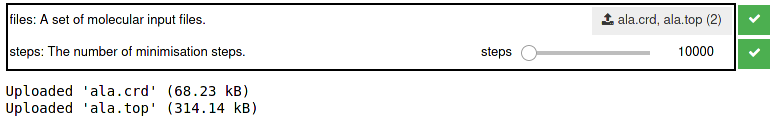
\includegraphics{https://github.com/michellab/BioSimSpaceTutorials/blob/c06201e9464732df5fd64fa560779ef333f59651/01_introduction/assets/04_gui.png}
\caption{Notebook GUI}
\end{figure}

Once all requirements are set then we can acces the values using the
\texttt{node.getInput} method. The first time this is called the
\texttt{node} will automatically validate all of the input and report
the user if any errors were found.

We'll now create a molecular system using the input files uploaded by
the user. As in the previous section, we don't need to specify the
format of the files, since this is automatically determined by
BioSimSpace. (BioSimSpace has support for a wide range of formats and
can convert between many formats too.)

\begin{Shaded}
\begin{Highlighting}[]
\NormalTok{system }\OperatorTok{=}\NormalTok{ BSS.IO.readMolecules(node.getInput(}\StringTok{"files"}\NormalTok{))}
\end{Highlighting}
\end{Shaded}

As learned in the previus notebook, in order to run a minimisation we
need to define a protocol. This can be done using the
\texttt{BSS.Protocol} package. Here we will create a ``best practice''
minimisation protocol, overriding the number of steps with the input
from the user.

\begin{Shaded}
\begin{Highlighting}[]
\NormalTok{protocol }\OperatorTok{=}\NormalTok{ BSS.Protocol.Minimisation(steps}\OperatorTok{=}\NormalTok{node.getInput(}\StringTok{"steps"}\NormalTok{))}
\end{Highlighting}
\end{Shaded}

We now have everything that is required to run a minimisation. To do so,
we use the \texttt{BSS.MD} package to find an appropriate molecular
dynamics package on our current environment. What package is found will
depend upon both the system and protocol, as well as the hardware that
is available to the user. (For example, the user can choose to find
packages with GPU support.)

Note that this is different to the previous section, where we
specifically launched AMBER and GROMACS processes ourselves. This is
what makes the node interoperable, i.e.~it will work regardles of what
MD packages are installed. (As long as we find a package that supports
minimisation and supports a molecular file format to which we can
convert the input system.) By adding the optional \texttt{engine}
requirement we have also allowed the user to override the \texttt{auto}
setting if they prefer to use a specific engine.

(By default, the \texttt{run} function automatically starts the process
so it will be running as once you execute the cell below.)

\begin{Shaded}
\begin{Highlighting}[]
\NormalTok{process }\OperatorTok{=}\NormalTok{ BSS.MD.run(system, protocol, engine}\OperatorTok{=}\NormalTok{node.getInput(}\StringTok{"engine"}\NormalTok{))}
\end{Highlighting}
\end{Shaded}

We now wait for the process to finish, then check whether there were any
errors before continuing. If errors were raised, then we raise an
exception and print the last 10 lines of stdout and stderr to the user.

\begin{Shaded}
\begin{Highlighting}[]
\NormalTok{process.wait()}

\ControlFlowTok{if}\NormalTok{ process.isError():}
    \BuiltInTok{print}\NormalTok{(process.stdout(}\DecValTok{10}\NormalTok{))}
    \BuiltInTok{print}\NormalTok{(process.stdout(}\DecValTok{10}\NormalTok{))}
    \ControlFlowTok{raise} \PreprocessorTok{RuntimeError}\NormalTok{(}\StringTok{"The process exited with an error!"}\NormalTok{)}
\end{Highlighting}
\end{Shaded}

When the process has finished running we can get the minimised molecular
configuration. We will save this to file using the same format as the
original system, and set the \texttt{minimised} output requirement to
the list of file names that were written.

\begin{Shaded}
\begin{Highlighting}[]
\NormalTok{node.setOutput(}\StringTok{"minimised"}\NormalTok{,}
\NormalTok{    BSS.IO.saveMolecules(}\StringTok{"minimised"}\NormalTok{, process.getSystem(), system.fileFormat()))}
\end{Highlighting}
\end{Shaded}

Finally, we validate that the node completed succesfully. This will
check that all output requirements are satisfied and that no errors were
raised by the user. Any file outputs will be available for the user to
download as a compressed archive.

Note that the validation will fail until the cell above finishes
running.

\begin{Shaded}
\begin{Highlighting}[]
\NormalTok{node.validate()}
\end{Highlighting}
\end{Shaded}

output.zip

Once we are satisfied with our node we can choosed to download it as a
regular Python script that can be run from the command-line.

In JupyterHub, click on: \texttt{File/Download\ As/Python}\\
In JupyterLab, click on:
\texttt{File/Export\ Notebook\ As/Export\ Notebook\ to\ Executable\ Script}

That's it, you've now succesfully executed your first BioSimSpace node!
